\definecolor{qqwuqq}{rgb}{0,0.39,0}
\definecolor{ffqqqq}{rgb}{1,0,0}
\definecolor{qqqqff}{rgb}{0,0,1}
\definecolor{qqttff}{rgb}{0,0.2,1}
\definecolor{zzttqq}{rgb}{0.6,0.2,0}
\definecolor{cqcqcq}{rgb}{0.75,0.75,0.75}
\begin{figure}[h!]
    \centering
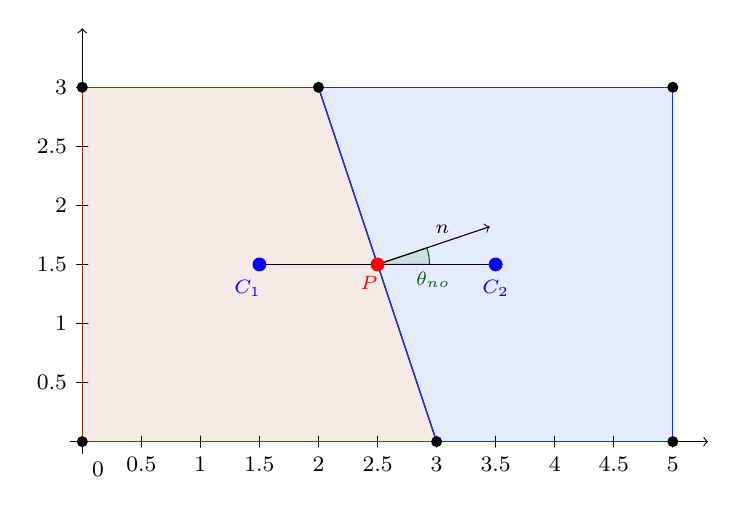
\begin{tikzpicture}[line cap=round,line join=round,x=1.5cm,y=1.5cm]
%\draw [color=cqcqcq,dash pattern=on 1pt off 1pt, xstep=0.5cm,ystep=0.5cm] (-0.1,-0.1) grid (5.3,3.5);
\draw[->,color=black] (-0.1,0) -- (5.3,0);
\foreach \x in {,0.5,1,1.5,2,2.5,3,3.5,4,4.5,5}
\draw[shift={(\x,0)},color=black] (0pt,2pt) -- (0pt,-2pt) node[below] {\footnotesize $\x$};
\draw[->,color=black] (0,-0.1) -- (0,3.5);
\foreach \y in {,0.5,1,1.5,2,2.5,3}
\draw[shift={(0,\y)},color=black] (2pt,0pt) -- (-2pt,0pt) node[left] {\footnotesize $\y$};
\draw[color=black] (0pt,-10pt) node[right] {\footnotesize $0$};
\clip(-0.1,-0.1) rectangle (5.3,3.5);
\fill[color=zzttqq,fill=zzttqq,fill opacity=0.1] (0,3) -- (0,0) -- (3,0) -- (2,3) -- cycle;
\fill[color=qqttff,fill=qqttff,fill opacity=0.1] (2,3) -- (3,0) -- (5,0) -- (5,3) -- cycle;
\draw [shift={(2.5,1.5)},color=qqwuqq,fill=qqwuqq,fill opacity=0.1] (0,0) -- (0:0.44) arc (0:18.43:0.44) -- cycle;
\draw (0,3)-- (0,0);
\draw (3,0)-- (0,0);
\draw (3,0)-- (2,3);
\draw (2,3)-- (0,3);
\draw (2,3)-- (5,3);
\draw (5,3)-- (5,0);
\draw (3,0)-- (5,0);
\draw [color=zzttqq] (0,3)-- (0,0);
\draw [color=zzttqq] (0,0)-- (3,0);
\draw [color=zzttqq] (3,0)-- (2,3);
\draw [color=zzttqq] (2,3)-- (0,3);
\draw [color=qqttff] (2,3)-- (3,0);
\draw [color=qqttff] (3,0)-- (5,0);
\draw [color=qqttff] (5,0)-- (5,3);
\draw [color=qqttff] (5,3)-- (2,3);
\draw (1.5,1.5)-- (3.5,1.5);
\draw [->] (2.5,1.5) -- (3.45,1.82);
\begin{scriptsize}
\fill [color=black] (0,3) circle (2.0pt);
\fill [color=black] (0,0) circle (2.0pt);
\fill [color=black] (3,0) circle (2.0pt);
\fill [color=black] (2,3) circle (2.0pt);
\fill [color=black] (5,3) circle (2.0pt);
\fill [color=black] (5,0) circle (2.0pt);
\fill [color=qqqqff] (1.5,1.5) circle (2.5pt);
\draw[color=qqqqff] (1.4,1.3) node {$C_1$};
\fill [color=qqqqff] (3.5,1.5) circle (2.5pt);
\draw[color=qqqqff] (3.5,1.3) node {$C_2$};
\fill [color=ffqqqq] (2.5,1.5) circle (2.5pt);
\draw[color=ffqqqq] (2.43,1.34) node {$P$};
\draw[color=black] (3.05,1.8) node {$n$};
\draw[color=qqwuqq] (2.97,1.37) node {$\theta_{no}$};
\end{scriptsize}
\end{tikzpicture}
    \caption{Non orthogonality.}
    \label{fig:nonOrtho}
\end{figure}
